\newpage
\appendix

\section{Alignment Prompts}
\label{appendix:align_prompt}

\subsection{Overview}
In this section we describe how we \textbf{align the world knowledge of a LLM with the SID space} so that the model can be directly used for generative recommendation.  

We append a three–layer codebook, each layer containing $256$ unique SIDs, to the original tokenizer vocabulary. The inserted codes are treated as indivisible tokens, enabling the LLM to read or write SID sequences without any sub-word splitting.
Then we introduce a set of auxiliary \emph{Alignment Tasks} to bridge the semantic gap between the textual vocabulary and the newly added SIDs. 
% These tasks repeatedly present the same item or user trace in two complementary views—plain text and SID sequences—so that the model is forced to learn a shared embedding space. 
A specialized \emph{Recommendation Tasks} further teach the model to predict the SID of the next item given an user history.

\subsection{Recommendation Tasks}

\begin{enumerate}
    \item \textbf{Generative Retrieval.} The main task ofor generative recommendation.  
    The LLM receives a chronologically ordered SID sequence that represents the user’s recent interactions, together with an explicit instruction such as “Recommend the next item.”, and is asked to predict the SID of the next item the user might engage with. A sample prompt is shown in the Figure \ref{fig:sid2sid}.

\begin{figure}[H]
    \centering
    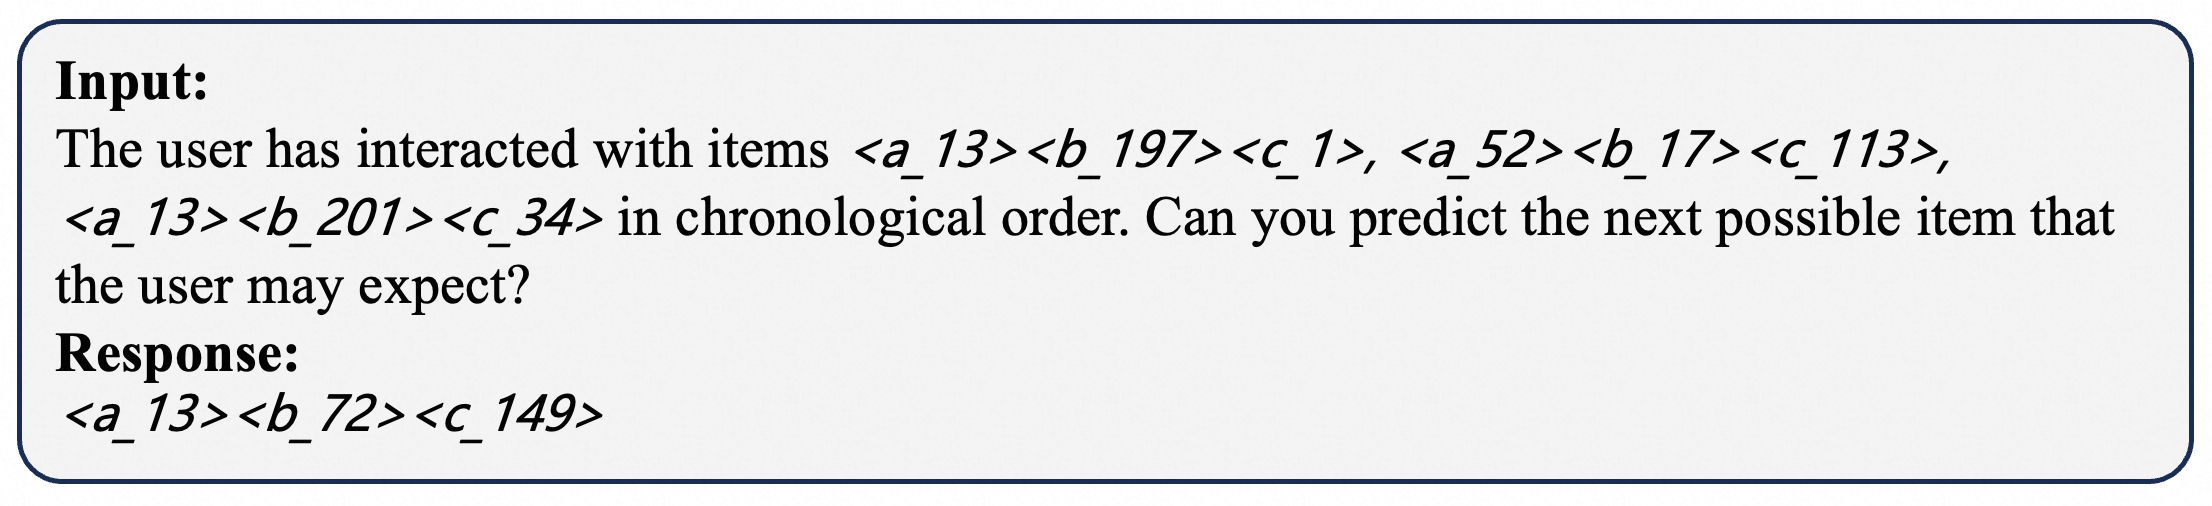
\includegraphics[width=0.8\textwidth]{figures/sid2sid.png}
    \vspace{-10pt}
    \caption{Generative Retrieval Prompt.}
    \label{fig:sid2sid}
    \vspace{-10pt}
\end{figure}

    \item \textbf{Asymmetric Item Prediction.}
    (a) Given a textual user history, predict the SID of the next item; (b) given a SID-only history, generate the textual title of the next item. Sample prompts are shown in the Figure \ref{fig:titlehis2sid} and Figure \ref{fig:sidhis2title}.

\begin{figure}[H]
    \centering
    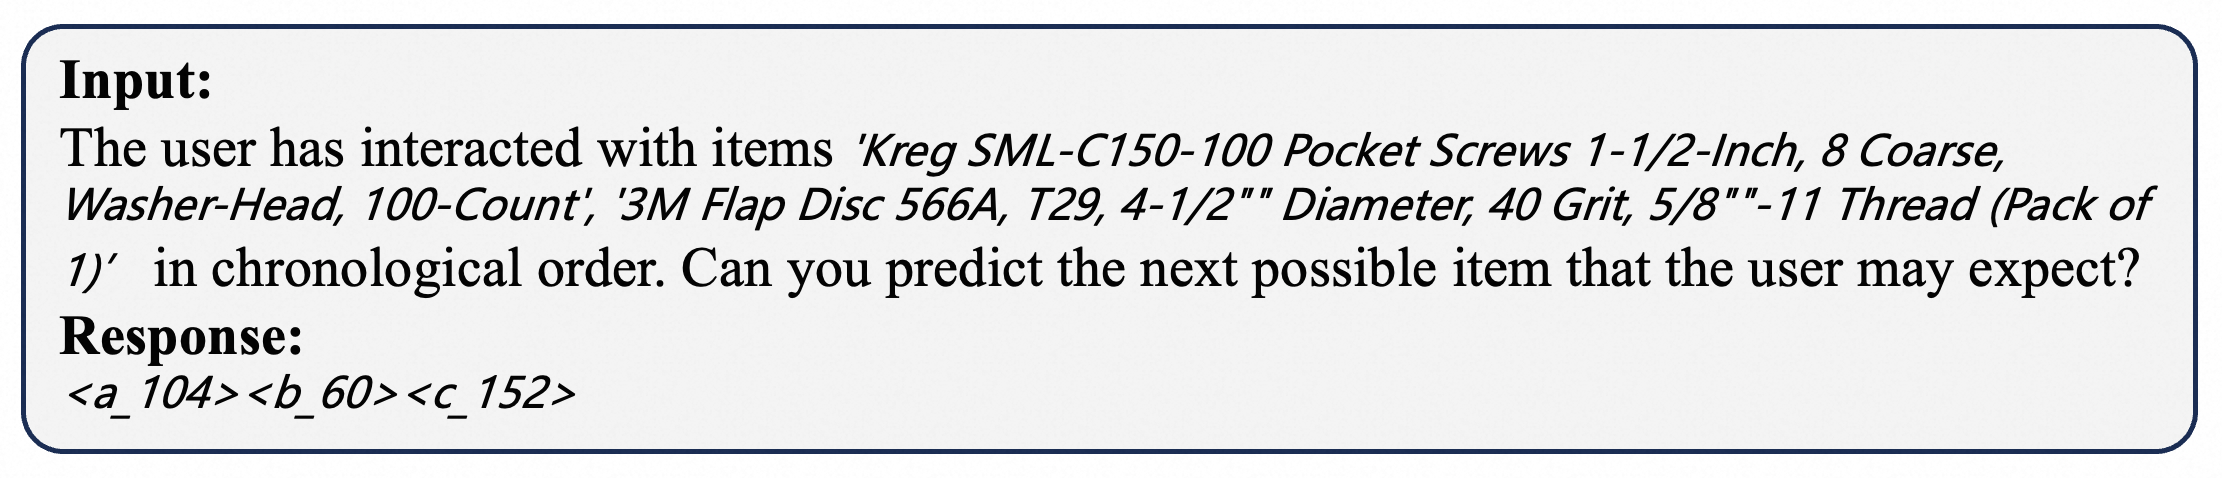
\includegraphics[width=0.8\textwidth]{figures/titlehis2sid.png}
    \vspace{-10pt}
    \caption{Asymmetric Item Prediction Prompt1.}
    \label{fig:titlehis2sid}
    \vspace{-10pt}
\end{figure}

\begin{figure}[H]
    \centering
    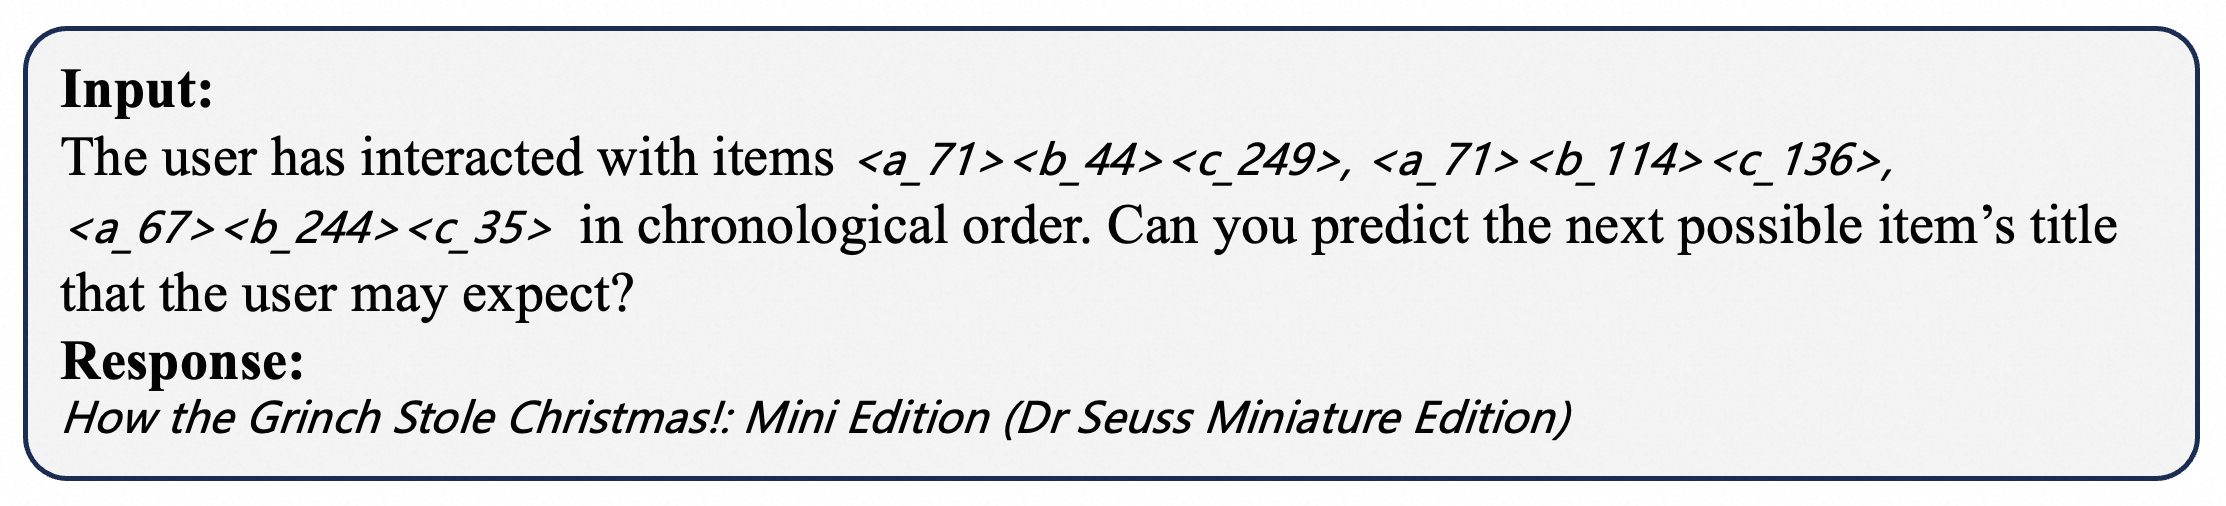
\includegraphics[width=0.8\textwidth]{figures/sidhis2title.png}
    \vspace{-10pt}
    \caption{Asymmetric Item Prediction Prompt2.}
    \label{fig:sidhis2title}
    \vspace{-10pt}
\end{figure}
\end{enumerate}

\subsection{Alignment Tasks}

\begin{enumerate}
    \item \textbf{SID–Text Semantic Alignment.} (a) Predict an item's textual title from its SID; (b) predict the SID from the item's textual title.  Sample prompts are shown in the Figure \ref{fig:sid2title} and Figure \ref{fig:title2sid}.

\begin{figure}[H]
    \centering
    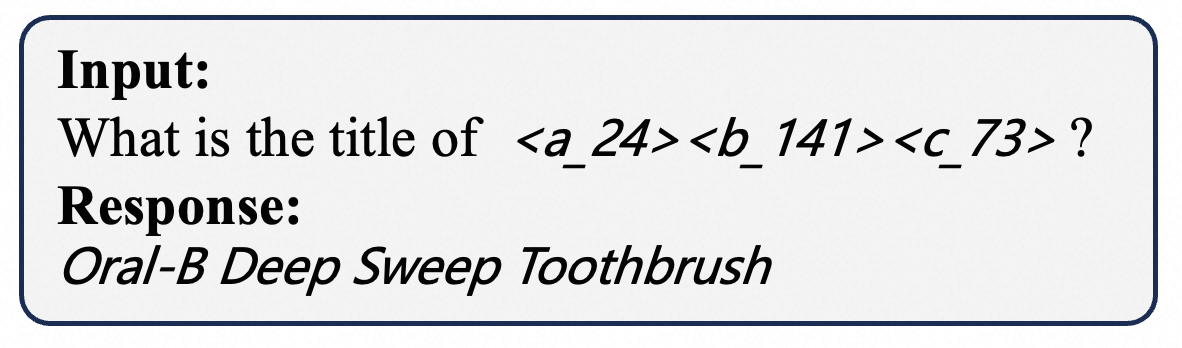
\includegraphics[width=0.45\linewidth]{figures/sid2title.png}
    \vspace{-10pt}
    \caption{SID–Text Semantic Alignment Prompt1.}
    \label{fig:sid2title}
    \vspace{-10pt}
\end{figure}

\begin{figure}[H]
    \centering
    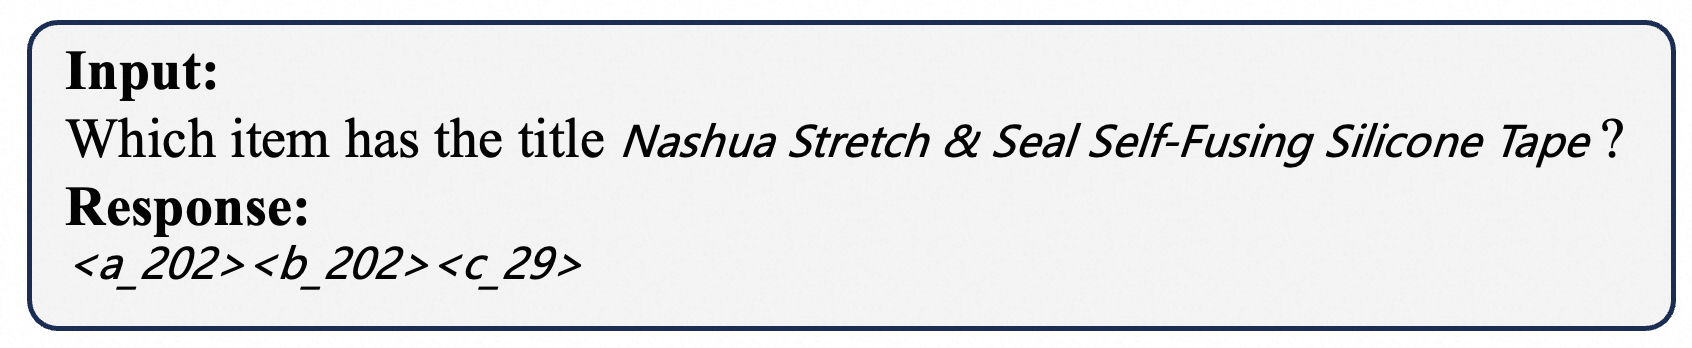
\includegraphics[width=0.64\textwidth]{figures/title2sid.png}
    \vspace{-10pt}
    \caption{SID–Text Semantic Alignment Prompt2.}
    \label{fig:title2sid}
    \vspace{-10pt}
\end{figure}

    \item \textbf{Item Description Reconstruction.}  
          To ground SIDs in richer semantics, we ask the model to generate the item description from a single SID and, conversely, infer the SID from the description. We perform this task only during the SFT stage because the description space is large and diverse. Sample prompts is shown in the Figure \ref{fig:description2sid}.

\begin{figure}[H]
    \centering
    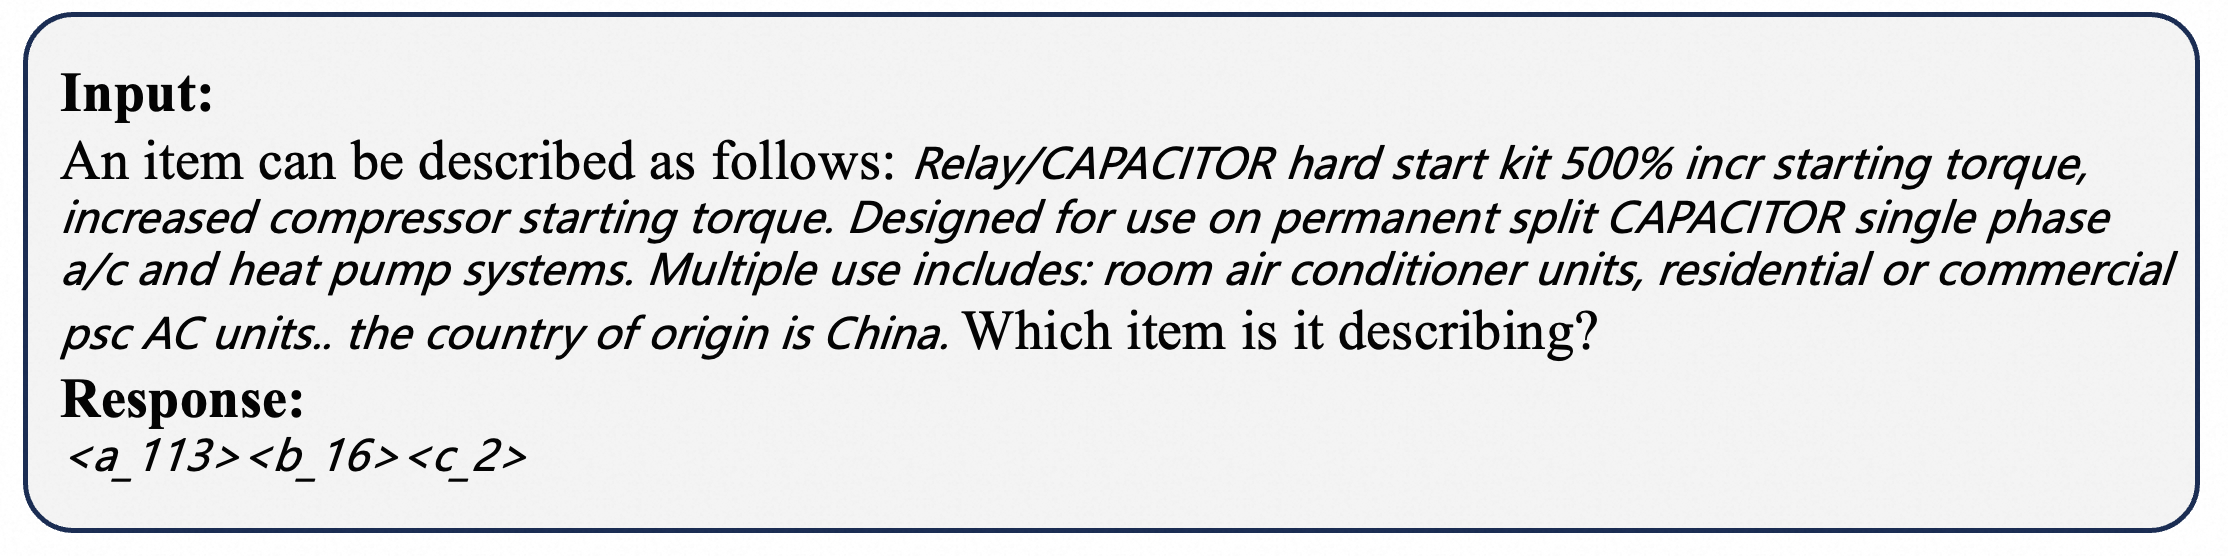
\includegraphics[width=0.8\textwidth]{figures/description2sid.png}
    \vspace{-10pt}
    \caption{Item Description Reconstruction Prompt.}
    \label{fig:description2sid}
    \vspace{-10pt}
\end{figure}

    \item \textbf{User Preference Summarization.}  
          Given a sequence of SIDs, the model produces a short natural–language profile that summarizes the user’s interests. Because the raw dataset lacks explicit preference labels, we employ \textsc{DeepSeek} \citep{deepseek} to extract summaries from the item's meta data and users’ textual reviews and use them as pseudo labels. This task, too, is restricted to the SFT stage due to the open-ended output space.
\begin{figure}[H]
    \centering
    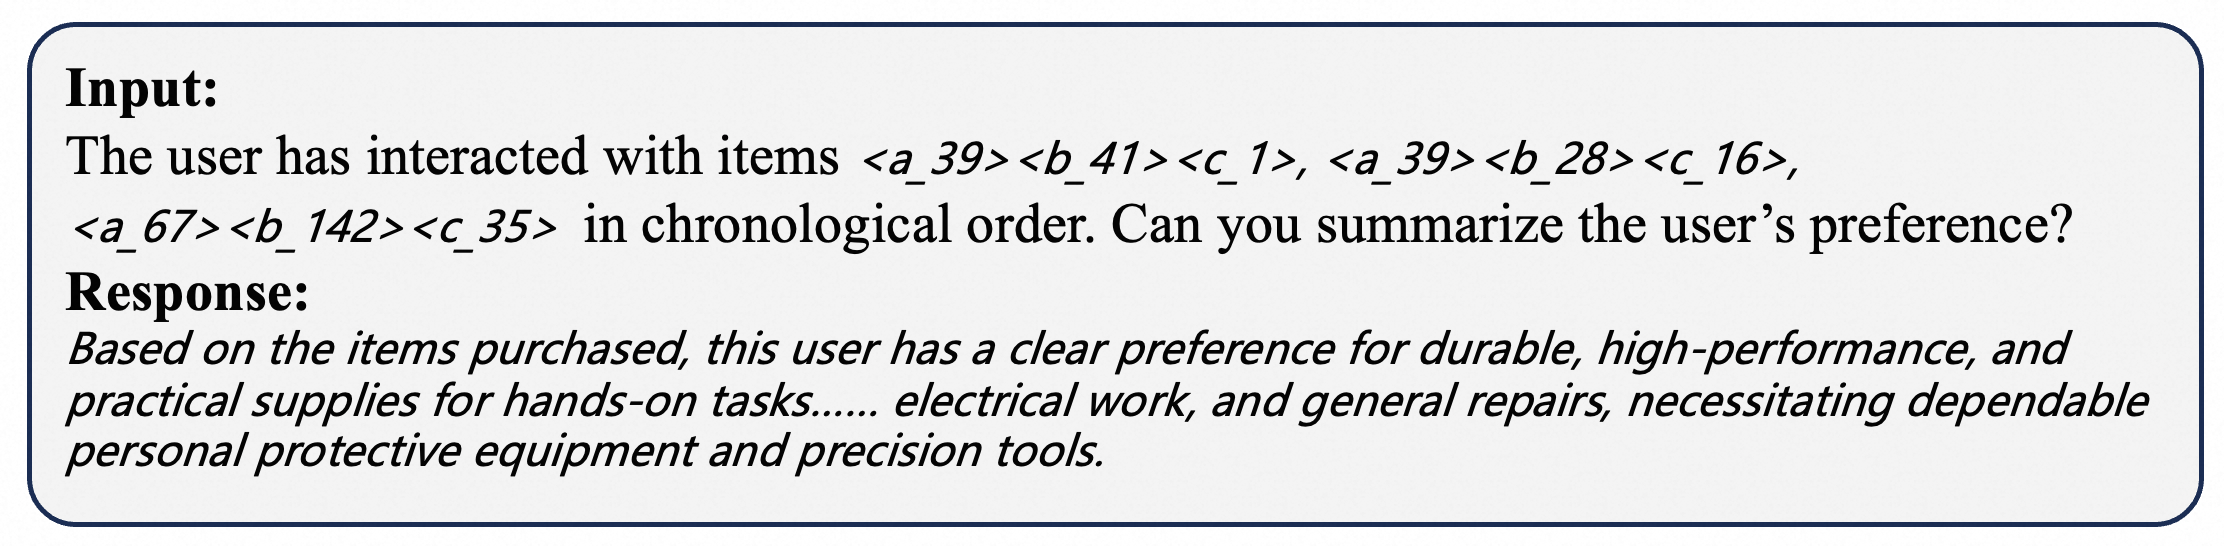
\includegraphics[width=0.8\textwidth]{figures/sidhis2preference.png}
    \vspace{-10pt}
    \caption{User Preference Summarization Prompt.}
    \label{fig:sid2title}
    \vspace{-10pt}
\end{figure}

\end{enumerate}


\section{Datasets}

We evaluate our model on two Amazon Review subsets:  Amazon Review subsets (\textit{Industrial\_and\_Scientific} and \textit{Office\_Products}).  
To keep computational costs affordable, we follow the trimming strategy used in \citep{D3}.  
The main steps are:  
(1) remove users and items with fewer than five interactions;  
(2) for \textit{Toys\_and\_Games}, keep events from October 2016 to November 2018;  
(3) for \textit{Industrial\_and\_Scientific}, which is smaller, keep all events between October 1996 and November 2018;   
(4) truncate every user history to at most ten items;  
(5) finally, split each dataset chronologically into training, validation and test sets with an 8:1:1 ratio.  
Key statistics of the resulting training splits are reported in Table~\ref{tab:stats}.

\begin{table}[H]
\centering
\caption{Statistics of datasets.} 
\label{tab:stats}
\begin{tabular}{ccc}
\toprule
Datasets & Inductrial & Office \\ \midrule
Items    & 3,685      & 3,459  \\
Train    & 3,6259     & 3,8924 \\
Valid    & 4,532      & 4,866  \\
Test     & 4,533      & 4,866  \\ \bottomrule
\end{tabular}
\end{table}